\scanpage{16}

Supposons en particulier
\[
B=A\otimes_k\Lambda
\]
où $\Lambda$ est une $k$-algèbre infinitésimale.
Alors \deleted{$\unsure{\Omega^1_\Lambda}$}
\[
\begin{aligned}
\mathfrak g_{B/\Lambda}\deleted{\unsure{(\Omega_\Lambda)}}
&=\operatorname{Hom}_B(\Omega^{\unsure{1|'}}_{B/\Lambda},B)
\simeq\operatorname{Hom}_B(\Omega^{\unsure{1|'}}_{A/k}\otimes_k\Lambda,A\otimes_k\Lambda)\\
&\simeq\operatorname{Hom}_A(\Omega^{\unsure{1|'}}_{A/k},A\otimes_k\Lambda)
\simeq\text{$k$-dérivations}\\
&\hspace{7cm}\text{de $A$ dans $A\otimes_k\Lambda$}
\end{aligned}
\]
et les $\Lambda$-dérivations de $B$ dans $B$ qui
induisent $0$ sur $B\otimes_\Lambda k\simeq\unsure{\Lambda|A}$ s'identifient
aux $k$-dérivations $A\;\text{---}\;A\otimes_k I(\Lambda)$.
Donc

\uline{Proposition} Supposons $k$ \deleted{\unsure{de}} $\supset\mathbb Q$, $A$ une
$k$-alg. comm., $\Lambda$ une $k$-alg. inf.
Alors \unsure{le|les} \inserted{groupe de} $\Lambda$-autom. infinitésimaux de
$A\otimes_k\Lambda$ \deleted{\unsure{sont en co}} est isomorphe
à l'ens des $k$-dérivations de
$A$ dans $A\otimes_k I(\Lambda)$, avec la structure
de groupe donnée par Hausdorff-
Campbell.
\figure{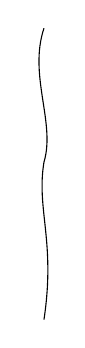
\begin{tikzpicture}\draw(0,0)..controls(.15,1)and(-.1,1.4)..(0,2)..controls(.15,2.5)and(-.2,3.1)..(0,3.7);\end{tikzpicture}}

\mspage{15}
